\documentclass[11pt, letterpaper]{article}
\usepackage{amsmath, amssymb}
\usepackage{booktabs}
\usepackage{geometry}
\usepackage{hyperref}
\usepackage{xcolor}
\usepackage{graphicx}
\usepackage{float}
\usepackage{enumitem}
\usepackage{tcolorbox}
\usepackage{algorithm}
\usepackage{algpseudocode}
\geometry{margin=1in}
\tcbuselibrary{skins, breakable}
\newtcolorbox{agentbox}[1]{title={#1}, colback=blue!3!white, colframe=blue!55!black,
  fonttitle=\bfseries, breakable}
\newtcolorbox{keybox}[1]{title={#1}, colback=green!3!white, colframe=green!45!black,
  fonttitle=\bfseries, breakable}
\newtcolorbox{warnbox}[1]{title={#1}, colback=orange!5!white, colframe=orange!70!black,
  fonttitle=\bfseries, breakable}
\hypersetup{colorlinks=true, linkcolor=blue!50!black}

\title{\textbf{Multi-Agent Receding-Horizon Games for Autonomous Market Participation}\\[4pt]
\large Detailed Case-Study Report --- Distributed Day-Ahead ADMM \& Explicit\\
Real-Time FACET Generalized Nash Equilibrium\\
\normalsize Green-H$_2$ coalition, ERCOT 2025, $H=4$ (1-hour) receding horizon, PCC band $[100,900]$ kW}
\author{Parth Brahmbhatt --- University of Wisconsin--Madison}
\date{\today}

\begin{document}
\maketitle
\tableofcontents
\bigskip\hrule\bigskip

\begin{abstract}
Six independently-owned green-hydrogen electrolyzers behind one point-of-common-coupling (PCC) bid
collectively into the ERCOT two-settlement market. \textbf{Both} market stages are solved fully
distributed, over the \emph{same} physical PCC import band $[L_{\min},L_{\max}]=[100,900]$~kW, and
\emph{no agent ever shares its cost model}. The day-ahead (DAM) anchor is set by a distributed
\textbf{ADMM} in which each agent solves only its own 24-hour QP and the sole shared quantity is
the per-hour coalition import. Real-time dispatch (RTM, 15-min) is a \textbf{receding-horizon}
($H=4$) parametric generalized Nash equilibrium (GNE) solved online by \textbf{FACET}: each agent
locates its own precomputed critical region by warm-started point-location over its facet-neighbour
graph (never enumerating the $K^N\!\approx\!9.7\times10^{20}$ combinations), the coalition combination
is made self-consistent, and the \emph{variational} GNE (= social optimum) is recovered by a
potential-minimizing solve that remains valid when the coupling binds. Over two independent ERCOT
weeks (1--7 April, 7--13 July 2025; $-\$1$ to $\$3553$/MWh) FACET clears \textbf{99.1\%} of steps
\emph{iteration-free} --- exactly one decision broadcast per agent per step --- meeting the weekly
H$_2$ target at \textbf{140--142\%}, holding renewable curtailment to \textbf{6.9--7.8\%} of available
generation, and matching the centralized equilibrium to $\sim\!10^{-4}$~kW in the interior. On the
$0.9\%$ of steps at the degenerate coupling ceiling a warm-started distributed ADMM fallback is used
(the only iteration). This report documents each agent's optimization problem, the distributed DAM
and the online FACET clearing step by step, and all measured results including curtailment.
\end{abstract}

\section{Physical system and market}
A cluster of small electrolyzers sits behind one shared PCC. Each owner runs its own asset for its
own revenue and keeps its cost model private; only power decisions are shared. Two forces make this
a game rather than $N$ independent problems:
\begin{itemize}[nosep]
\item \textbf{Physical coupling.} The PCC caps the collective import and a market floor sets a
minimum offer, \emph{at every 15-min step $k$}:
\[
   L_{\min}=100\ \text{kW}\ \le\ \sum_{i=1}^{N} p_{i,k}\ \le\ L_{\max}=900\ \text{kW}.
\]
$L_{\min}$ is the ISO minimum offer size; $L_{\max}$ is the physical interconnection limit
($75\%$ of the $1200$~kW fleet nameplate). \textbf{This same band governs both the day-ahead and the
real-time stage} --- there is one physical wire.
\item \textbf{Private hydrogen contracts.} Each agent must produce a daily H$_2$ quantity; it may
time production freely but the daily total is a hard floor. That freedom, under a shared per-step
power limit, is what couples the agents and the horizon.
\end{itemize}
The market is ERCOT two-settlement: a day-ahead (DAM, hourly) stage that sets a financial anchor
$p^{\mathrm{DA}}$, and a real-time (RTM, 15-min SCED) stage that re-optimizes against live prices.
Electricity $\to$ H$_2$ conversion: $\text{kg}=\eta_i\,p_{\mathrm{elec},i}\,\Delta t$, $\Delta t=0.25$~h.

\section{The fleet (medium-scale)}
\begin{table}[H]\centering
\begin{tabular}{clcccccc}
\toprule
$i$ & Agent & type & $P_{\max,i}$ & renew.\ cap & $\eta_i$ & $\gamma_i$ & break-even $a_i$\\
 & & & [kW] & [kW] & [kg/kWh] & & [\$/MWh]\\
\midrule
0 & PEM\_Elec  & grid & 250 & --  & 0.020 & $5\!\times\!10^{-3}$ & 60\\
1 & ALK        & grid & 200 & --  & 0.018 & $5\!\times\!10^{-3}$ & 54\\
2 & PEM\_PV    & PV   & 125 & 125 & 0.020 & $5\!\times\!10^{-3}$ & 60\\
3 & PEM\_PV\_2 & PV   & 125 & 125 & 0.020 & $5\!\times\!10^{-3}$ & 60\\
4 & PEM\_Wind  & wind & 250 & 250 & 0.020 & $4\!\times\!10^{-3}$ & 60\\
5 & PEM\_Wind\_2 & wind & 250 & 250 & 0.020 & $4\!\times\!10^{-3}$ & 60\\
\bottomrule
\end{tabular}
\caption{$N=6$, total nameplate $1200$~kW. $r_{\mathrm{H2}}=\$3$/kg, $H=4$, $\Delta t=0.25$~h.
Break-even $a_i=r_{\mathrm{H2}}\eta_i\!\cdot\!10^3$: below $a_i$ buying grid power to make H$_2$ is
profitable, above it the agent wants to stop. Agents 2--3 and 4--5 are identical pairs (they share
one offline solve each).}
\end{table}

% ─────────────────────────────────────────────────────────────────────────────
\section{Day-Ahead stage: distributed ADMM (model-private)}\label{sec:dam}
% ─────────────────────────────────────────────────────────────────────────────
The day-ahead schedule is solved once per day on the DAM \emph{forecast}
($\hat\lambda_h=\lambda^{\mathrm{DA}}_h+\mathcal N(0,16)$, renewable $\hat g_{i,h}$). It is
\textbf{distributed}: each agent $i$ solves only its own 24-hour problem, and the \emph{only}
exchanged quantity is the per-hour coalition import $\sum_i p_{i,h}$ (already public at the metered
point). No agent reveals $P_{\max,i}$, $\eta_i$, its renewable cap, or its daily target.

\paragraph{Per-agent day-ahead problem.} With $\Delta t_{\mathrm{DA}}=1$~h and daily target
$D^{\mathrm{day}}_i=0.55\,P_{\max,i}\eta_i\!\cdot\!24$, agent $i$ solves
\[
\min_{p_{i,h}\ge0,\;cv_{i,h}\ge0}\ \sum_{h=0}^{23}\Big[(\hat\lambda_h/1000-r_{\mathrm{H2}}\eta_i)\,
   \Delta t_{\mathrm{DA}}\,p_{i,h}+r_{\mathrm{H2}}\eta_i\,\Delta t_{\mathrm{DA}}\,cv_{i,h}
   +\underbrace{\tfrac12\gamma_{\mathrm{DA}}\,p_{i,h}^2}_{\text{regularizer}}\Big]
\]
\[
\begin{aligned}
&0\le p_{i,h}\le P_{\max,i},\quad 0\le cv_{i,h}\le \mathrm{cap}_i \qquad\text{(local box; $cv$ only renewables)}\\
&0\ \le\ p_{i,h}+\hat g_{i,h}-cv_{i,h}\ \le\ P_{\max,i} \qquad\text{(local renewable balance)}\\
&\textstyle\sum_{h=0}^{23}\eta_i\,(p_{i,h}+\hat g_{i,h}-cv_{i,h})\,\Delta t_{\mathrm{DA}}\ \ge\ D^{\mathrm{day}}_i
   \qquad\text{(hard daily H$_2$ floor)}
\end{aligned}
\]
Every term uses only agent $i$'s own data; the daily H$_2$ floor couples that agent's own 24 hours.
The \textbf{coupling band} $L_{\min}\le\sum_i p_{i,h}\le L_{\max}$ ($\forall h$) is the \emph{only}
cross-agent constraint, enforced by ADMM consensus/dual updates that see nothing but the per-hour
aggregate:
\[
\text{(x)}\ p_i^{\ell+1}=\arg\min\big[J_i(p_i)+\tfrac{\rho}{2}\|p_i-z_i^\ell\|^2\big],\quad
\text{(z)}\ z^{\ell+1}=\Pi_{[L_{\min},L_{\max}]}\!\big(\textstyle\sum_i p_i^{\ell+1}+\mu^\ell/\rho\big),\quad
\text{($\mu$)}\ \mu_i^{\ell+1}=\mu_i^{\ell}+\rho(p_i^{\ell+1}-z_i^{\ell+1}),
\]
with $\rho=0.1$; $\Pi$ is a closed-form clip of the per-hour aggregate onto the band. The award
$p^{\mathrm{DA}}_{i,h}$ is the RTM anchor; its cumulative-H$_2$ trajectory sets the RTM pacing target
$D_i(t)$. (\texttt{dam.solve\_dam\_admm}; consensus in \texttt{admm\_solver.py}.)

\begin{keybox}{The small $\gamma_{\mathrm{DA}}$ regularizer (why, and its trade-off)}
The day-ahead economics are \emph{linear} in each hourly buy: ``buy enough cheap power to make the
day's hydrogen.'' With no $\gamma_{\mathrm{DA}}$ the problem is a degenerate LP --- on a cheap day it
says \emph{buy the maximum every hour}, a knife-edge answer that ADMM oscillates on and cannot
settle. A \emph{tiny} quadratic penalty $\tfrac12\gamma_{\mathrm{DA}}p_{i,h}^2$
($\gamma_{\mathrm{DA}}=10^{-4}$) rounds the knife-edge: it spreads purchases smoothly, gives a
\emph{unique} schedule so ADMM converges, and changes total cost by $\le\!1.4\%$. A matching
$\varepsilon=10^{-3}$ regularizes renewable curtailment $cv$. Validation: a centralized solve of the
\emph{same} regularized problem (offline oracle, \texttt{solve\_dam\_centralized}) is matched to
$\le\!10$~kW on priced days; on ultra-flat days the day-ahead problem is genuinely degenerate so the
two solvers land on different equally-optimal schedules ($\le\!23$~kW apart, cost within $1\%$).
\end{keybox}

% ─────────────────────────────────────────────────────────────────────────────
\section{Real-Time stage: each agent's mpQP}
% ─────────────────────────────────────────────────────────────────────────────
Every RTM step, agent $i$ solves a strictly-convex mpQP over the horizon $k=0,\dots,3$. The decision
is grid import $p_{i,k}\ge0$ (renewable agents additionally choose curtailment $cv_{i,k}$). The cost
is a day-ahead deviation anchor $\tfrac12\gamma_i(p-p^{\mathrm{DA}}_i)^2$ (strict convexity,
$Q_i\succ0$) plus real-time energy cost net of H$_2$ revenue. \textbf{Each agent's cost and every
local constraint use only that agent's own parameters; the sole shared quantity is the aggregate
$\mathrm{s}_k=\sum_{j\ne i}p_{j,k}$.}

\subsection{Grid agents (PEM\_Elec $i{=}0$, ALK $i{=}1$)}
\begin{agentbox}{Grid agent $i$ --- decision $x_i=[p_{i,0..3}]\in\mathbb R^4$}
\textbf{Private parameters} $\theta_i=[\,\mathrm{s}_0..\mathrm{s}_3\mid D_i,\ \lambda_0..\lambda_3,\ p^{\mathrm{DA}}_i\,]\in\mathbb R^{10}$
\[
\min_{p_i\in\mathbb R^4}\ \sum_{k=0}^{3}\Big[\tfrac12\gamma_i\,(p_{i,k}-p^{\mathrm{DA}}_i)^2
   +\big(\lambda_k/1000-r_{\mathrm{H2}}\eta_i\big)\,\Delta t\;p_{i,k}\Big]
\]
\vspace{-8pt}
\[
\begin{aligned}
&0\le p_{i,k}\le P_{\max,i}, &&\text{(capacity box)}\\
&\textstyle\sum_{k}\eta_i\,p_{i,k}\,\Delta t\ \ge\ D_i, &&\text{(cumulative H$_2$ --- couples the 4 steps)}\\
&L_{\min}\ \le\ p_{i,k}+\mathrm{s}_k\ \le\ L_{\max}. &&\text{(shared per-step coupling)}
\end{aligned}
\]
\end{agentbox}

\subsection{Renewable agents (PEM\_PV $i{=}2,3$; PEM\_Wind $i{=}4,5$)}
Renewable output $g_{i,k}$ feeds the electrolyzer load $p_{\mathrm{elec},i,k}=p_{i,k}+g_{i,k}-cv_{i,k}$
(free renewable displaces grid import; curtailment $cv$ throws away H$_2$ at break-even).
\begin{agentbox}{Renewable agent $i$ --- decision $x_i=[p_{i,0..3},\,cv_{i,0..3}]\in\mathbb R^8$}
\textbf{Private parameters} $\theta_i=[\,\mathrm{s}_0..\mathrm{s}_3\mid D_i,\ \lambda_0..\lambda_3,\ p^{\mathrm{DA}}_i,\ g_0..g_3\,]\in\mathbb R^{14}$
\[
\min_{p_i,cv_i}\ \sum_{k=0}^{3}\Big[\tfrac12\gamma_i(p_{i,k}-p^{\mathrm{DA}}_i)^2+\tfrac12\varepsilon\,cv_{i,k}^2
  +(\lambda_k/1000-r_{\mathrm{H2}}\eta_i)\Delta t\,p_{i,k}+r_{\mathrm{H2}}\eta_i\,\Delta t\,cv_{i,k}\Big]
\]
\vspace{-8pt}
\[
\begin{aligned}
&0\le p_{i,k}\le P_{\max,i},\quad 0\le cv_{i,k}\le g_{i,k}\le\mathrm{cap}_i,\\
&0\ \le\ p_{\mathrm{elec},i,k}=p_{i,k}+g_{i,k}-cv_{i,k}\ \le\ P_{\max,i},\\
&\textstyle\sum_{k}\eta_i\,p_{\mathrm{elec},i,k}\,\Delta t\ \ge\ D_i,\qquad
L_{\min}\ \le\ p_{i,k}+\mathrm{s}_k\ \le\ L_{\max}\ \text{(grid import only)}.
\end{aligned}
\]
\end{agentbox}

\paragraph{Receding-horizon coupling (not a repeated static game).} The four steps couple only
through the cumulative-H$_2$ row. At an H$_2$-binding point (PEM, raise $\lambda_1$ by \$40/MWh):
$\Delta p=[+0.5,-1.5,+0.5,+0.5]$~kW with $\sum_k p_k:600\to600$ (H$_2$-conserved). Step~1 becomes
expensive so it drops; the others rise to keep the H$_2$ total --- a single-step map would give
$\Delta p=\mathbf0$.

\paragraph{Sum-compression and elimination.} Agent $i$ depends on the others only through the
per-step aggregate $\mathrm{s}_k=\sum_{j\ne i}p_{j,k}$ (4 numbers), not their private
$D_j,p^{\mathrm{DA}}_j,g_j$. Each agent's mpQP is solved offline (PPOPT) in its private $10$- or
$14$-dimensional $\theta_i$; the coupling variable is eliminated when the coalition combination is
assembled. Public parameter count is $4(\lambda)+6(p^{\mathrm{DA}})+6(D)+8(g)=24$, but no
24-dimensional problem is ever solved.

The daily pacing target is receding: $D_i(t)=\text{clip}\big((D^{\mathrm{day}}_i-h2^{\mathrm{inv}}_i)\,
H/\text{steps left in day},\,0,\,D^{\max}_i\big)$; only step $k=0$ is executed against realized price
and renewable, then the window advances.

% ─────────────────────────────────────────────────────────────────────────────
\section{Online FACET clearing of the RTM GNE}\label{sec:facet}
% ─────────────────────────────────────────────────────────────────────────────
Each agent's offline solution is an explicit piecewise-affine map: a set of \emph{critical regions}
(CRs), each a polytope $E_i\theta_i\le f_i$ carrying an affine law $x_i=G_i\theta_i+g_i$. A
\emph{combination} $\mathcal C=(r_0,\dots,r_5)$ picks one CR per agent; the equilibrium at combination
$\mathcal C$ solves a block-linear system $M_x x = M_p\theta+M_1$. FACET finds and solves the correct
combination online \textbf{without enumerating the $K^N\!\approx\!9.7\times10^{20}$ combinations}.

\begin{keybox}{The FACET method (what runs every 15-minute step)}
\begin{enumerate}[leftmargin=1.6em,nosep]
\item \textbf{Per-agent point-location (warm-started).} Each agent locates its own CR at
$[\mathrm{s}_i;\theta]$ using the \emph{previous} step's CR as a hint: test that CR and its
facet-neighbours first (\,$\approx\!50$ checks\,); only on a miss does a vectorized scan over that
agent's own CRs run. This is per-agent (thousands of CRs), never over combinations.
\item \textbf{Self-consistent coalition combination.} Assemble the located CRs into a combination;
re-locate each agent given the others' aggregate and iterate to a fixed point --- a genuine GNE
(each agent best-responding to the shared aggregate).
\item \textbf{Variational-GNE solve.} Solve $M_x x=M_p\theta+M_1$ by the \emph{potential-minimizing}
selection: when the coupling binds for $\ge2$ agents $M_x$ is rank-deficient (a manifold of
equilibria); we pick the one minimizing the coalition potential $\sum_i J_i$ = the variational GNE =
social optimum (matches the centralized oracle). A plain solve would fail on that singular system.
\item \textbf{Facet-neighbour walk (backup).} If the located combination is not yet a strict
equilibrium, walk the combination's facet-neighbour graph (1st/2nd/3rd neighbour) for the closest
valid one; a 1-hop min-potential refinement locks the variational combination.
\item \textbf{ADMM fallback (rare; the only iteration).} If steps 1--4 fail --- only at genuinely
degenerate ceiling vertices --- fall back to a warm-started distributed ADMM solve. Its result is
used only if it converges; a non-converged result never becomes a warm start.
\end{enumerate}
All of steps 1--4 are \emph{local computation on the onboard maps}: the inter-agent exchange is
\textbf{exactly one decision broadcast per agent per step}, regardless of how many local checks run.
\end{keybox}

\begin{keybox}{Privacy model (no centralized optimizer at either stage)}
Agents share \textbf{only their bidding decisions, never their cost models} --- in both the DAM
(\S\ref{sec:dam}) and the RTM (\S\ref{sec:facet}). Consequently no party can solve the joint problem
at runtime. A centralized QP is used \textbf{only offline} to certify accuracy (map $=$ centralized)
and to bound an iterative solver's round count; it is never in the loop.
\end{keybox}

\subsection{The multiparametric maps (built once, offline)}
Each agent's RTM mpQP is solved \emph{once, offline} in its private parameter space $\theta_i$ by a
combinatorial multiparametric-QP solver (PPOPT). The result is the explicit piecewise-affine map:
a set of critical regions (CRs), each a polytope $E_i\theta_i\le f_i$ carrying an affine control law
$x_i=G_i\theta_i+g_i$. Only \textbf{4 distinct solves} are needed --- the two PV agents and the two
wind agents are identical --- then expanded into the six agent slots. Crucially, the private
$\theta_i$ box spans the \emph{full} operating range of every parameter --- price
$\lambda\in[-50,300]$, day-ahead anchor $p^{\mathrm{DA}}_i\in[0,P_{\max,i}]$, demand
$D_i\in[0,D^{\max}_i]$, renewable $g$ --- so the \emph{same} maps are valid for \emph{every} day and
\emph{every} DAM anchor. \textbf{The RTM maps are therefore built exactly once, never rebuilt}; only
the day-ahead ADMM runs daily.

\begin{table}[H]\centering
\begin{tabular}{llccr}
\toprule
Agent & type & $\dim\theta_i$ & decision $x_i$ & CRs\\
\midrule
PEM\_Elec         & grid       & 10 & $[p_{0..3}]\in\mathbb R^4$        & 507\\
ALK               & grid       & 10 & $[p_{0..3}]\in\mathbb R^4$        & 507\\
PEM\_PV, PEM\_PV\_2 & renewable & 14 & $[p_{0..3},cv_{0..3}]\in\mathbb R^8$ & 8359 (each)\\
PEM\_Wind, PEM\_Wind\_2 & renewable & 14 & $[p_{0..3},cv_{0..3}]\in\mathbb R^8$ & 7335 (each)\\
\midrule
\textbf{Total} & & & & \textbf{32{,}402} (4 distinct solves)\\
\bottomrule
\end{tabular}
\caption{Offline multiparametric maps: per-agent critical-region counts. Each agent solves its own
$10$- or $14$-dimensional mpQP; $\theta_i$ is compressed by the coupling ``sum'' variable so no
$24$-dimensional problem is ever solved. One-time offline cost $\approx\!13$~min; facet-neighbour
graphs $\approx\!1$~s. \textbf{Generated once} and reused for both entire weeks.}
\label{tab:cr}
\end{table}

% ─────────────────────────────────────────────────────────────────────────────
\section{Results --- two 7-day runs (ERCOT 2025)}
% ─────────────────────────────────────────────────────────────────────────────
Both weeks use the full $[100,900]$ band at both stages and the deployed FACET clearing
(1 broadcast/step). ``map $=$ cent'' is the max over the certified steps of
$\|x_{\mathrm{FACET}}-x_{\mathrm{centralized}}\|_\infty$; ``fallbacks'' are steps that needed the
warm-started ADMM escape; curtailment is renewable generation that could not be absorbed.

\begin{table}[H]\centering
\begin{tabular}{lrrrrr}
\toprule
Day & $\lambda_{\mathrm{RT}}$ [\$/MWh] & map $=$ cent [kW] & ADMM fallbacks & H$_2$ met & curtail [kWh]\\
\midrule
04-01 & $10$--$73$   & $2.6\!\times\!10^{-4}$ & 0 & 167\% & 748\\
04-02 & $17$--$282$  & $2.1$                  & 1 & 122\% & 342\\
04-03 & $11$--$31$   & $6.9\!\times\!10^{-6}$ & 0 & 134\% & 275\\
04-04 & $9$--$60$    & $6.4\!\times\!10^{-6}$ & 1 & 139\% & 300\\
04-05 & $11$--$23$   & $5.9$                  & 0 & 163\% & 716\\
04-06 & $-1$--$234$  & $5.5$                  & 0 & 131\% & 765\\
04-07 & $0$--$3553$  & $3.4$                  & 1 & 126\% & 236\\
\midrule
\textbf{Week 1 (1--7 Apr)} & & \textbf{$\le5.9$} & \textbf{3/672} & \textbf{140\%} & \textbf{3381}\\
\bottomrule
\end{tabular}
\caption{\textbf{Week 1.} 3 fallbacks / 672 steps ($99.6\%$ iteration-free). Interior days match the
centralized equilibrium to $\sim\!10^{-6}$--$10^{-4}$~kW; boundary days (ceiling-bound) sit within
$\le5.9$~kW ($<\!1\%$ of $900$) of the social optimum --- the multi-equilibrium residual of
\S\ref{sec:limit}. Weekly curtailment $3381/43380$~kWh $=7.8\%$ of available renewable.}
\end{table}

\begin{table}[H]\centering
\begin{tabular}{lrrrrr}
\toprule
Day & $\lambda_{\mathrm{RT}}$ [\$/MWh] & map $=$ cent [kW] & ADMM fallbacks & H$_2$ met & curtail [kWh]\\
\midrule
07-07 & $22$--$95$   & $1.9$ & 1 & 135\% & 165\\
07-08 & $21$--$151$  & $4.2$ & 1 & 132\% & 102\\
07-09 & $17$--$98$   & $4.9$ & 1 & 148\% & 181\\
07-10 & $11$--$79$   & $2.6$ & 4 & 156\% & 448\\
07-11 & $12$--$1754$ & $1.6$ & 1 & 163\% & 803\\
07-12 & $26$--$312$  & $0.32$ & 1 & 132\% & 434\\
07-13 & $16$--$82$   & $3.2$ & 0 & 129\% & 256\\
\midrule
\textbf{Week 2 (7--13 Jul)} & & \textbf{$\le4.9$} & \textbf{9/672} & \textbf{142\%} & \textbf{2390}\\
\bottomrule
\end{tabular}
\caption{\textbf{Week 2 (summer, unseen).} 9 fallbacks / 672 ($98.7\%$ iteration-free), including a
$\$1754$ scarcity spike (07-11). Weekly curtailment $2390/34540$~kWh $=6.9\%$.}
\end{table}

\begin{table}[H]\centering
\begin{tabular}{lrr|rr}
\toprule
& \multicolumn{2}{c|}{\textbf{Week 1 (April)}} & \multicolumn{2}{c}{\textbf{Week 2 (July)}}\\
Agent & H$_2$ / target [kg] & curtail / avail [kWh] & H$_2$ / target [kg] & curtail / avail [kWh]\\
\midrule
PEM\_Elec      & $608/462$ (132\%) & --- (grid) & $620/462$ (134\%) & --- (grid)\\
ALK            & $418/333$ (126\%) & --- (grid) & $408/333$ (123\%) & --- (grid)\\
PEM\_PV (each) & $335/231$ (145\%) & $372/3521$  & $358/231$ (155\%) & $499/6043$\\
PEM\_Wind (each) & $681/462$ (147\%) & $1318/18169$ & $679/462$ (147\%) & $696/11227$\\
\bottomrule
\end{tabular}
\caption{Per-agent weekly H$_2$ and curtailment. Every agent meets its contract (the receding
$D_i(t)$ pacing keeps all on or above target); over-production ($>\!100\%$) reflects the day-ahead
buying cheap power at the ceiling when $\lambda<a_i$. Renewable curtailment stays $\le\!8\%$ of
available generation: the coalition lets renewable-rich agents absorb their own output rather than
being forced to curtail. Rows ``each'' report one agent of the identical pair.}
\end{table}

\subsection{Critical-region and combination usage over the 2-week run}
The number of \emph{combinations} (one CR per agent) is
$K^N=507^2\cdot8359^2\cdot7335^2\approx9.7\times10^{20}$ --- impossible to enumerate; FACET never
does. Over the $1344$ real-time steps of both weeks, FACET selected only \textbf{619 distinct
combinations} --- a fraction $6.4\times10^{-19}$ of the possible set --- and operation concentrates
on a handful: the single most-used combination is selected on $117$ of $1344$ steps. This empirical
concentration ($\sim\!50$--$90$ distinct combinations per day out of $10^{21}$) is exactly what
FACET's neighbour-graph walk exploits, and why the $32{,}402$-CR maps of Table~\ref{tab:cr} never
need enumerating.

\begin{table}[H]\centering
\begin{tabular}{lccc}
\toprule
& Week 1 (April) & Week 2 (July) & Both weeks\\
\midrule
Distinct combinations per day & 48--67 & 53--86 & ---\\
Distinct combinations over the week & 322 & 394 & ---\\
\textbf{Distinct combinations used (union)} & & & \textbf{619}\\
Of $K^N\approx9.7\times10^{20}$ possible & & & $6.4\times10^{-19}$\\
Real-time steps & 672 & 672 & 1344\\
Most-used combination (visits) & & & 117 / 1344\\
\bottomrule
\end{tabular}
\caption{Combination usage. Of $\sim\!10^{21}$ possible combinations, real operation lives on
\textbf{619} recurring ones over two weeks --- the maps (Table~\ref{tab:cr}) are built once and the
FACET walk visits only this tiny recurring set.}
\end{table}

\paragraph{Communication / data transfer.} Every map step exchanges exactly \textbf{one decision
broadcast per agent} (the FACET location, walk and refinement are local). Only the rare ADMM-fallback
steps carry iterative rounds. Over each week the map steps contribute $1$ round/step; the $3$
(April) / $9$ (July) fallback steps contribute the remaining rounds. An iterative GNE seeker
run on \emph{every} step would instead need $\sim\!10^2$--$10^3$ agent broadcasts per step.

\subsection{Figures}
\begin{figure}[H]\centering
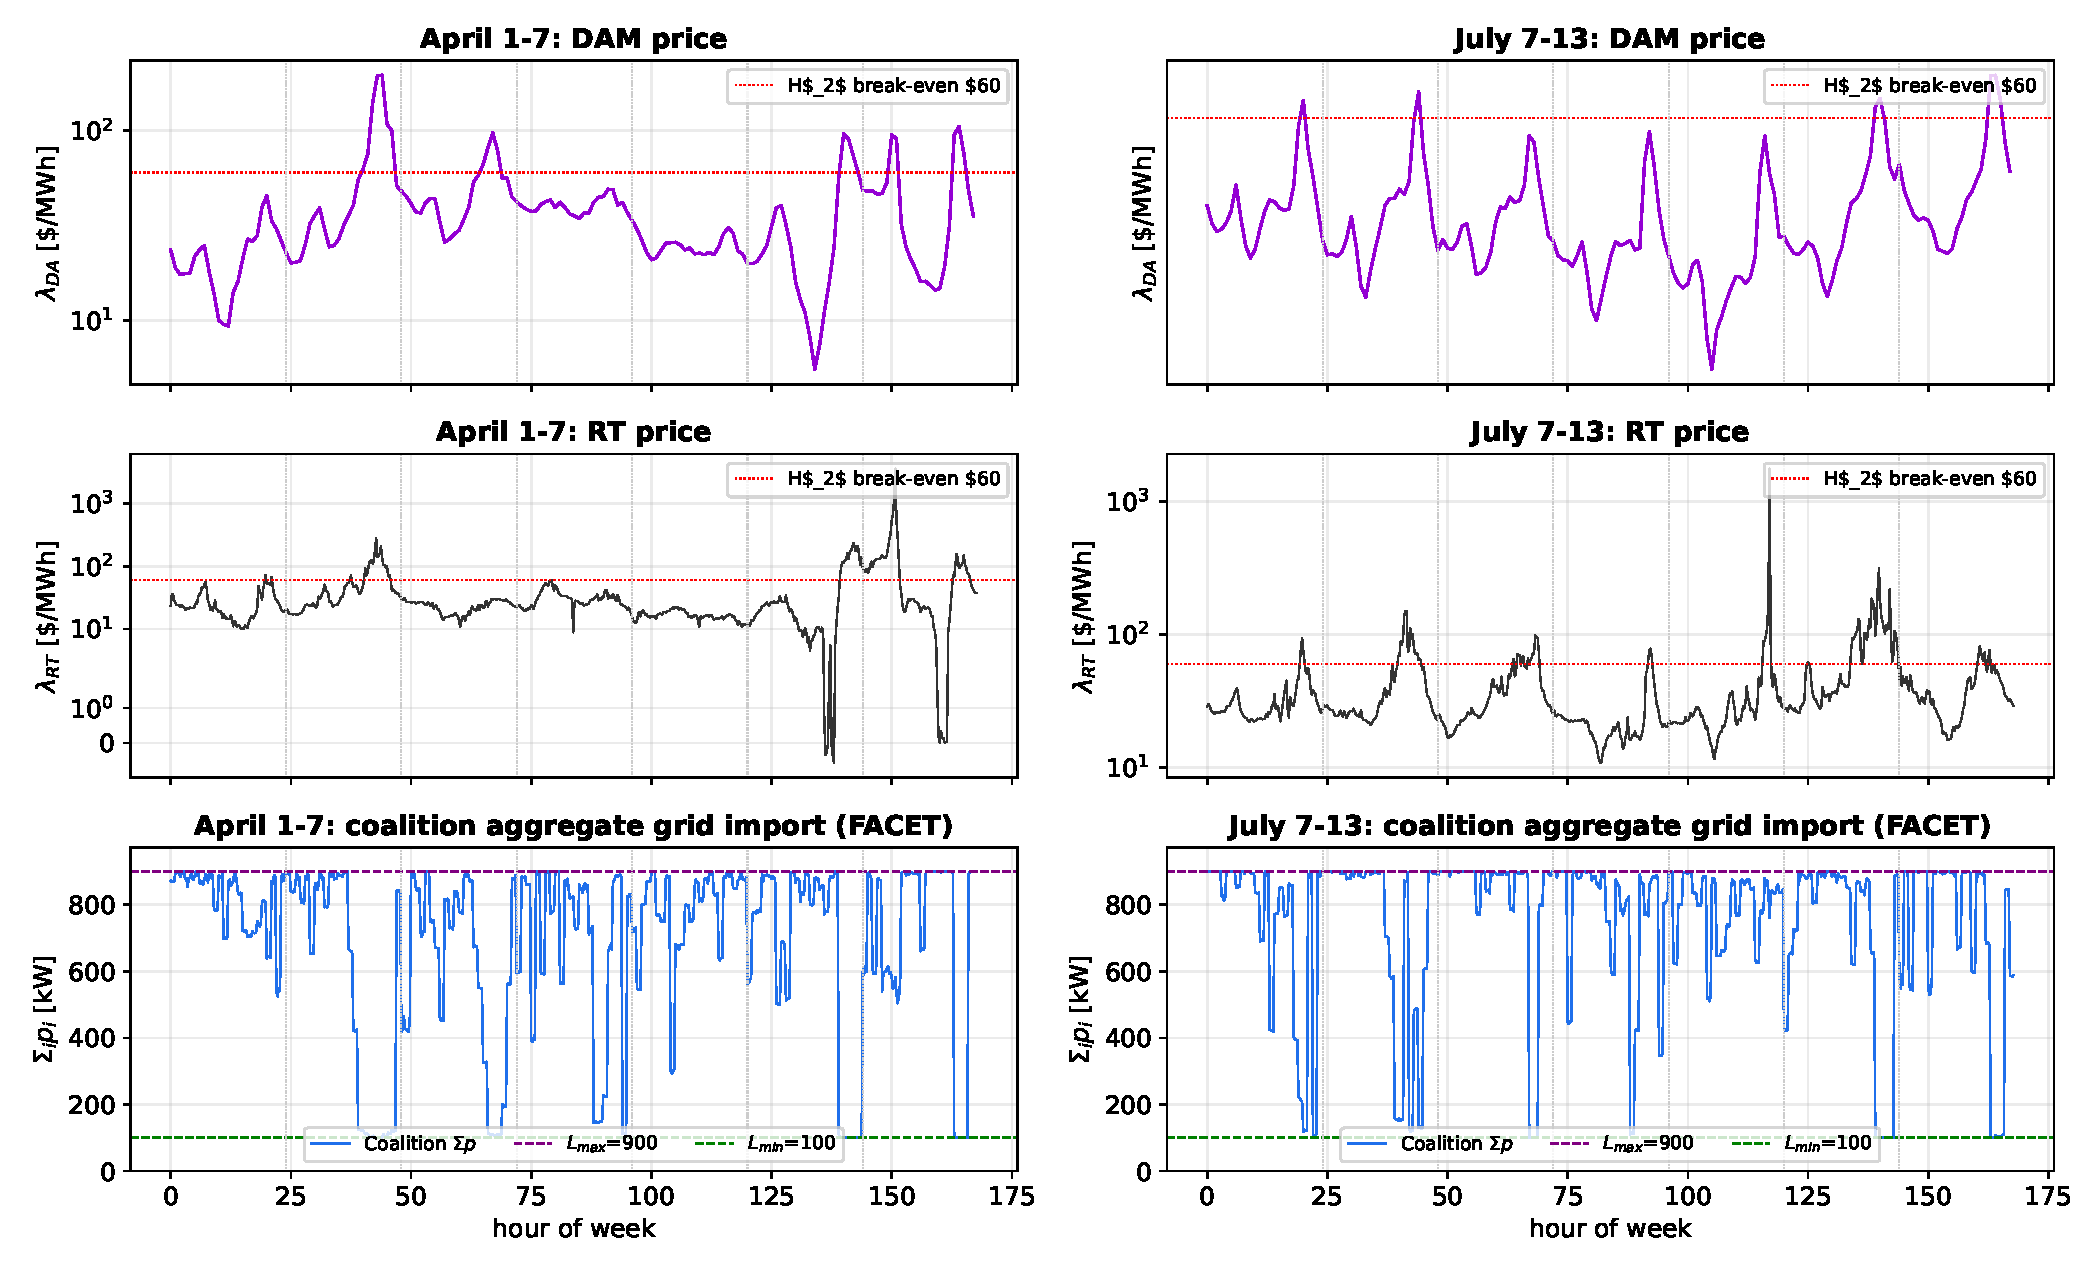
\includegraphics[width=\textwidth]{../results/figures/report/fig1_weekly_aggregate.pdf}
\caption{Coalition aggregate grid import $\Sigma_i p_i$ (bottom) against the RT price (top, symlog)
over each week, from the FACET clearing. The aggregate stays within $[L_{\min},L_{\max}]=[100,900]$
(dashed) at all times; it rides the ceiling on cheap hours (buy H$_2$) and retreats when the RT price
exceeds the H$_2$ break-even.}
\end{figure}
\begin{figure}[H]\centering
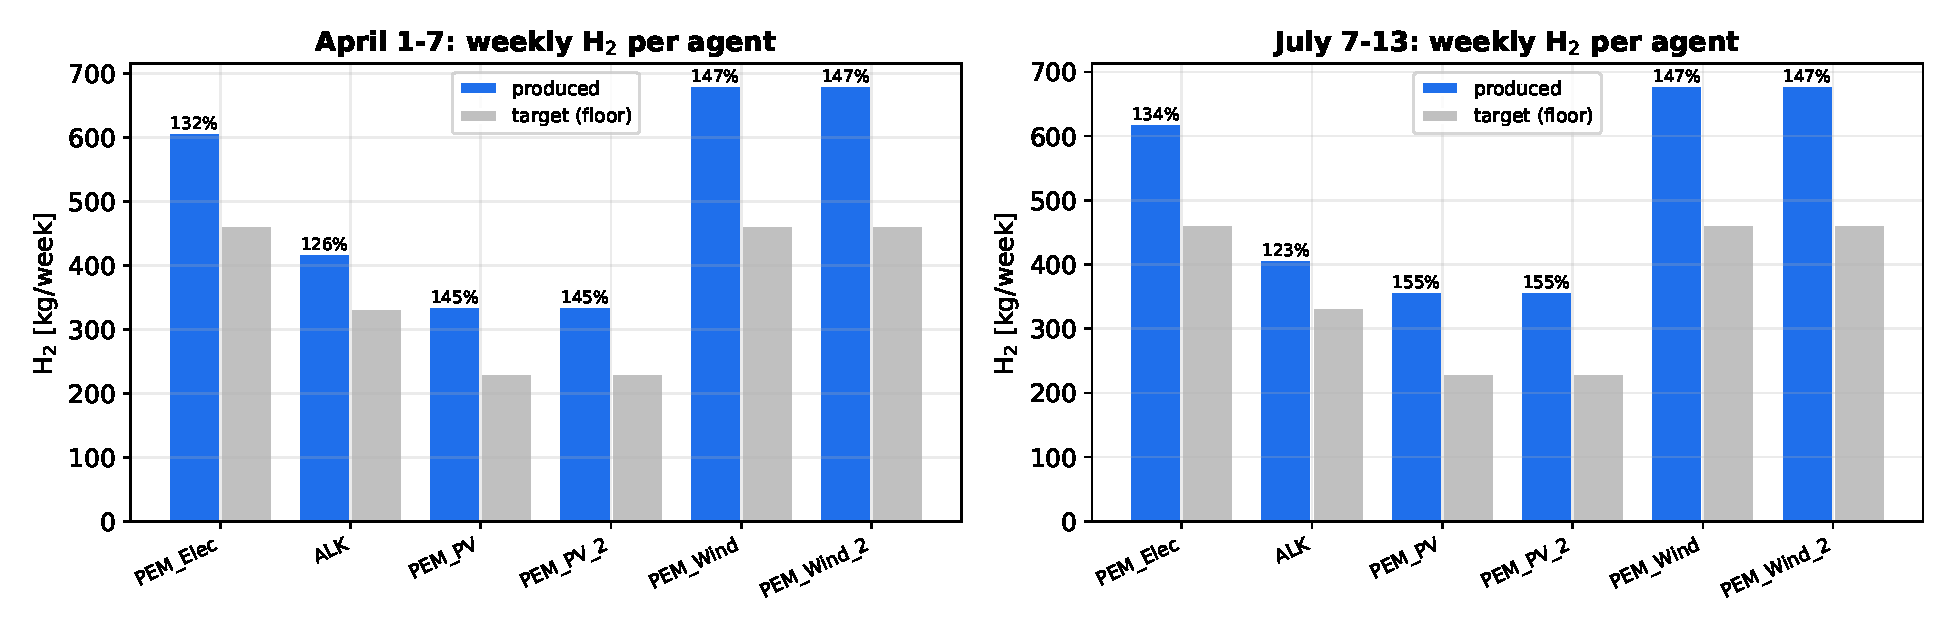
\includegraphics[width=\textwidth]{../results/figures/report/fig2_h2_per_agent.pdf}
\caption{Weekly H$_2$ per agent, produced vs.\ the contract floor (target). Every agent clears its
floor; over-production reflects buying cheap power at the ceiling. Labels show \% of target.}
\end{figure}
\begin{figure}[H]\centering
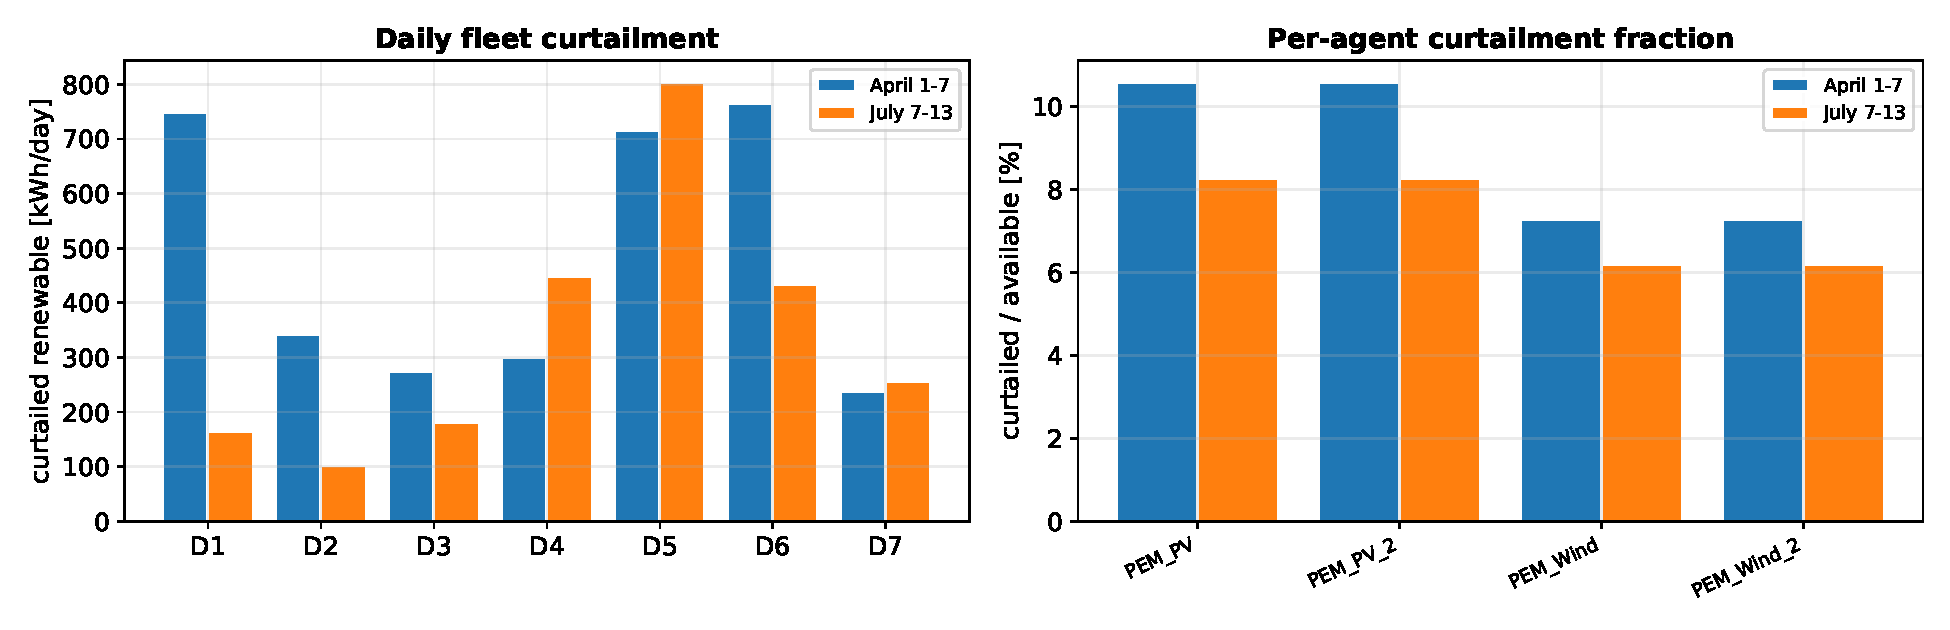
\includegraphics[width=\textwidth]{../results/figures/report/fig3_curtailment.pdf}
\caption{Left: daily fleet renewable curtailment (kWh) for both weeks. Right: per-agent curtailment
as a fraction of available renewable --- $\le\!8\%$: the coalition lets renewable-rich agents absorb
their own output rather than being forced to curtail.}
\end{figure}
\begin{figure}[H]\centering
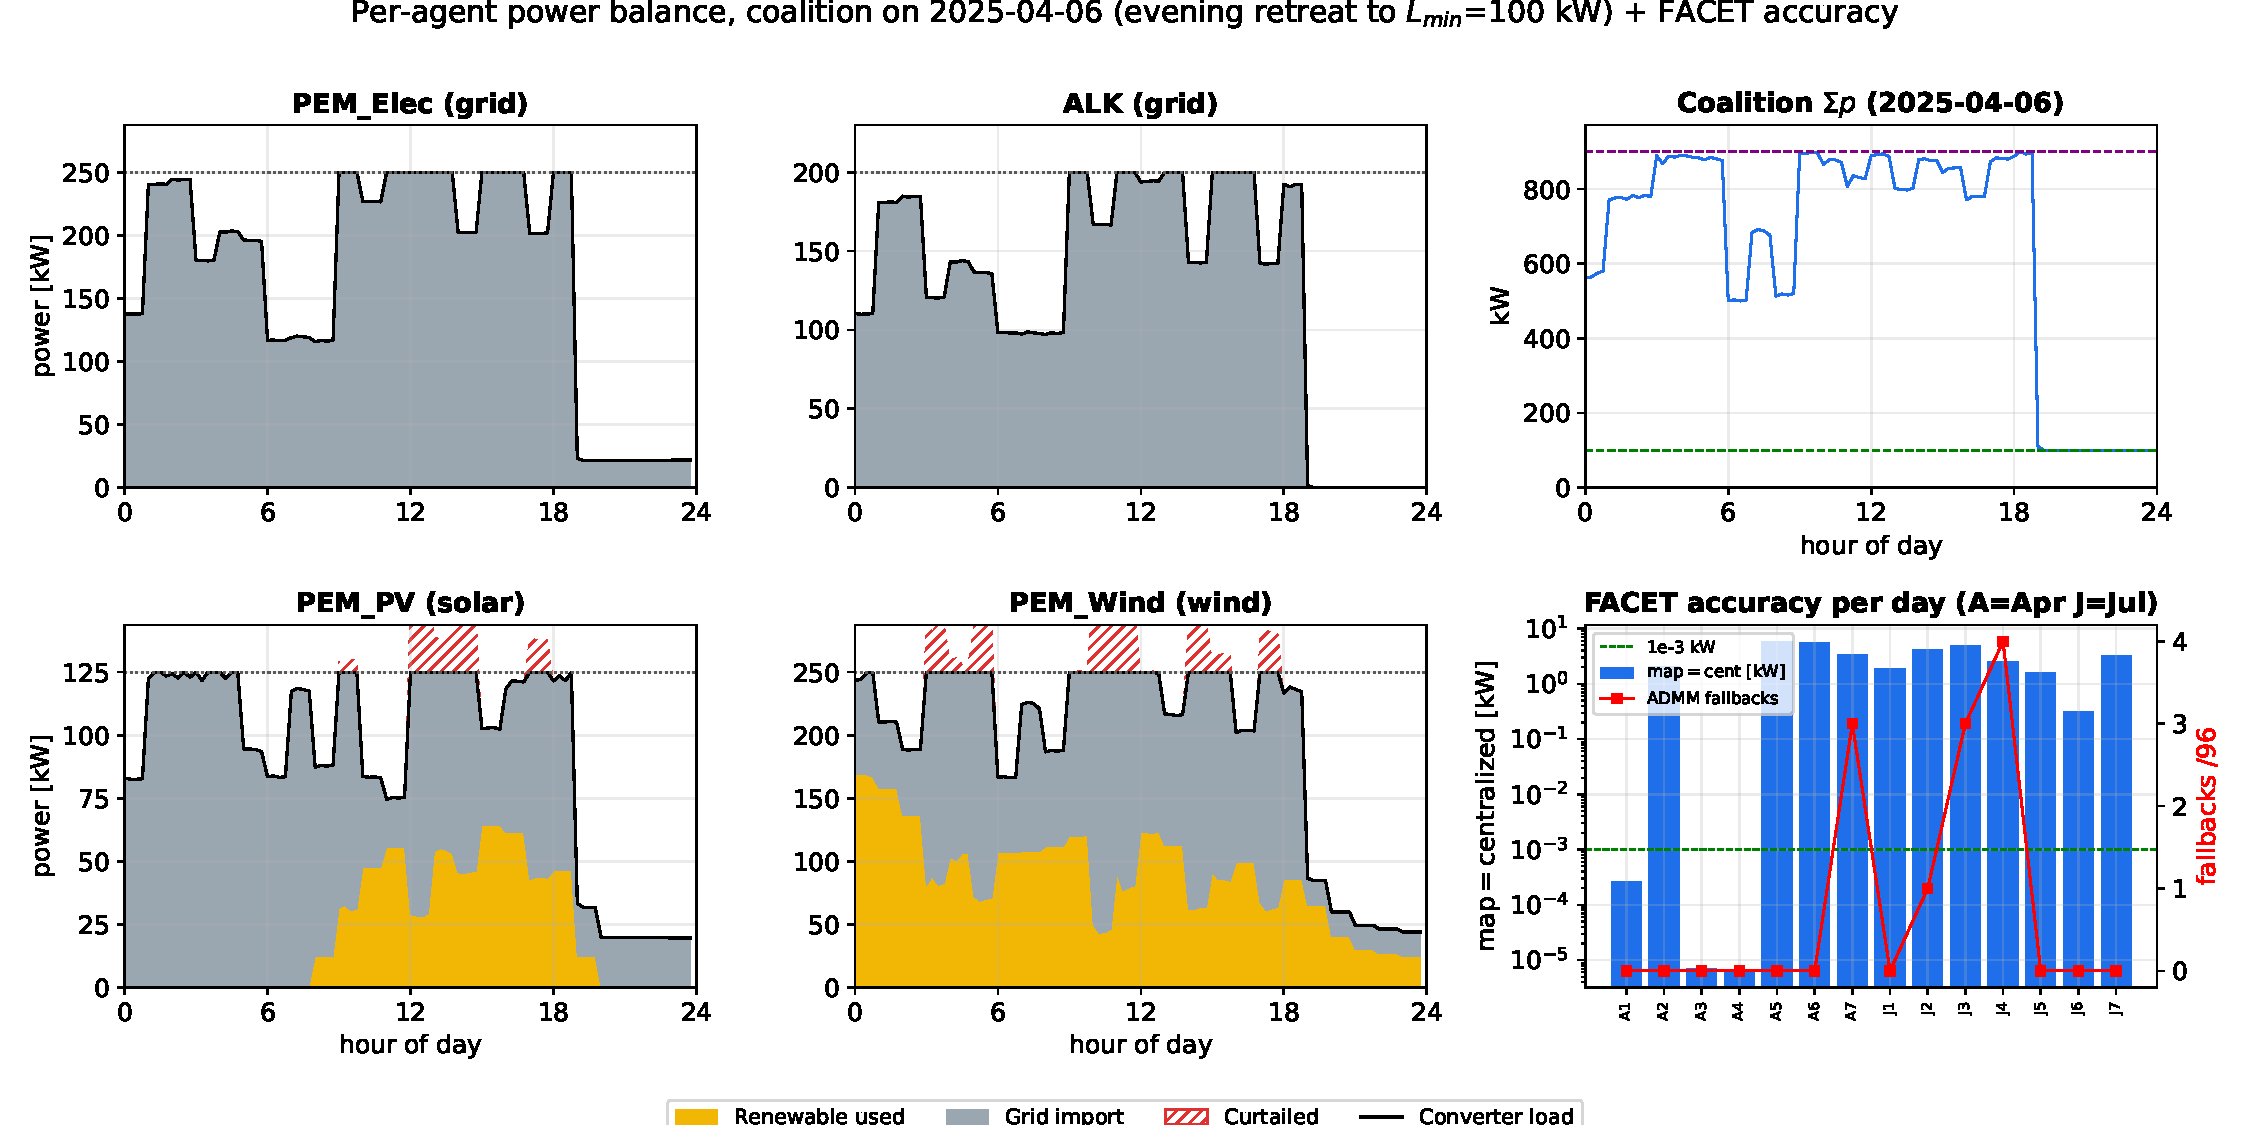
\includegraphics[width=\textwidth]{../results/figures/report/fig4_mechanism.pdf}
\caption{Per-agent power balance on 2025-04-06 (coalition) --- a day the RT price swings from
$-\$1$ to $\$234$/MWh, so the coalition both rides the ceiling (cheap/negative hours) \emph{and}
\textbf{retreats to $L_{\min}=100$~kW when expensive}: the renewable agents opt out of the market
(grid import $\to0$, running on their own generation, gold) while the grid agents cover the floor
(top-right aggregate touches $100$). The converter load (black) $=$ renewable used (gold) $+$ grid
import (grey); curtailed renewable is the red hatch above the load. Bottom-right: FACET accuracy
(map $=$ centralized, log, bars) and ADMM fallbacks (red) per day across both weeks --- interior days
$\sim\!10^{-6}$~kW, ceiling-bound days a few kW, fallbacks $\le\!4/96$.}
\end{figure}
\begin{figure}[H]\centering
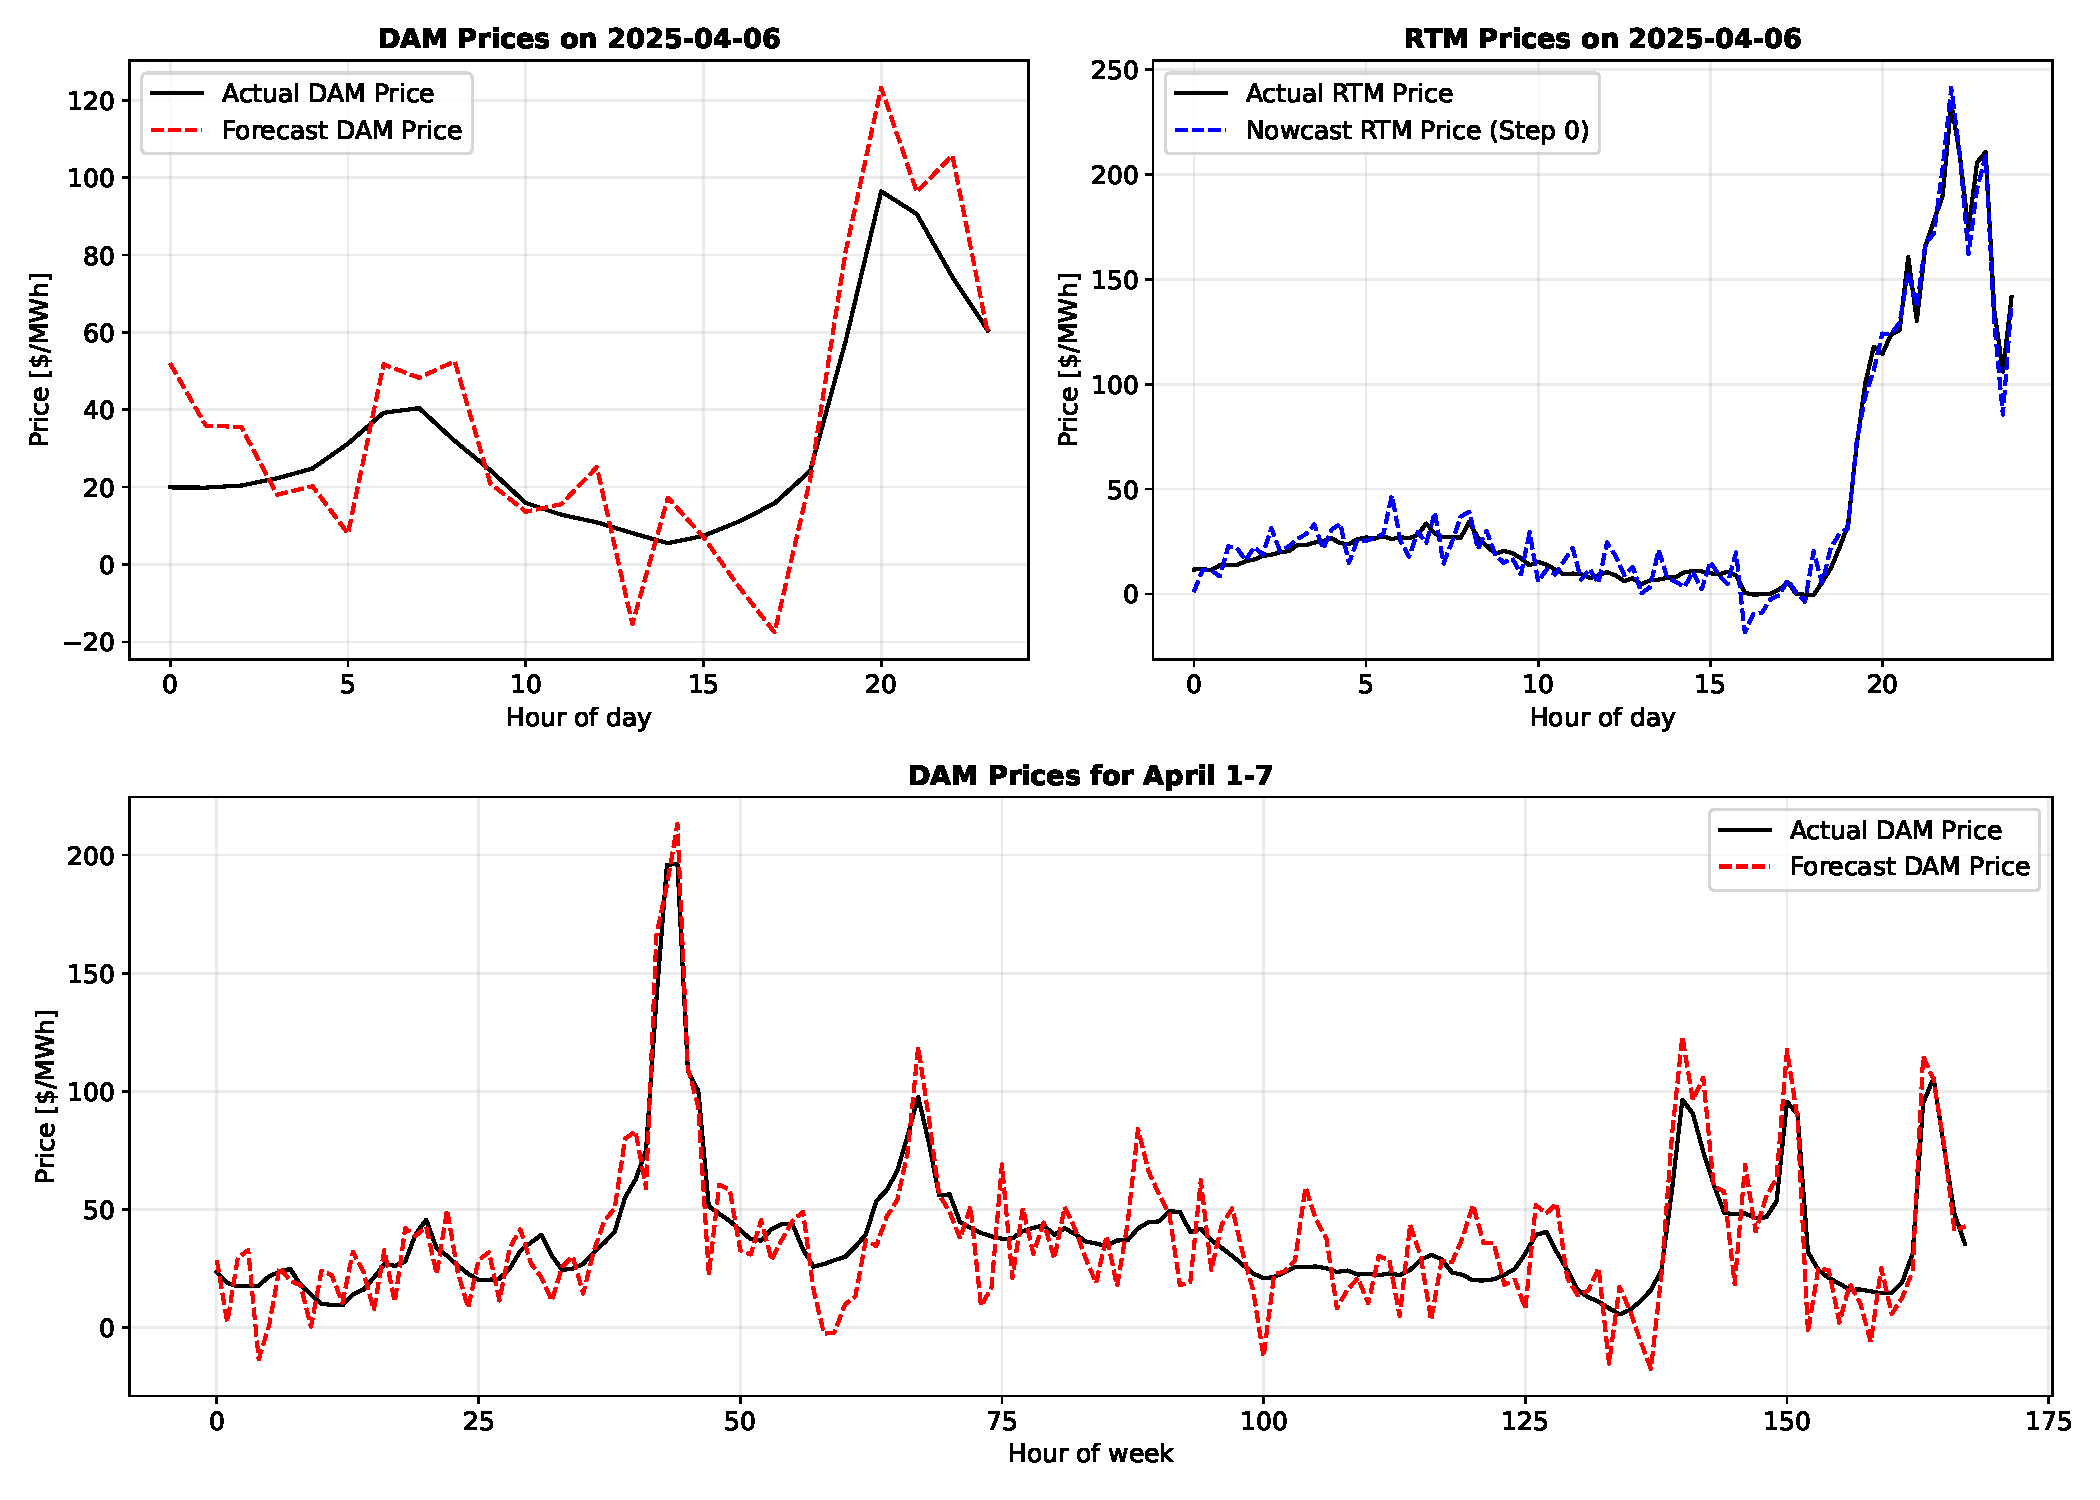
\includegraphics[width=\textwidth]{../results/figures/report/fig5_prices.pdf}
\caption{Actual vs.\ forecasted prices for the DAM (top left) and RTM (top right) on a representative
day (2025-04-06), and the DAM prices for the entire week (bottom). The DAM forecast is evaluated
once, a day ahead; the RTM nowcast is re-evaluated at every 15-minute receding step with fresh noise
--- illustrating the forecast-vs-realized split the RTM must correct for online.}
\end{figure}

% ─────────────────────────────────────────────────────────────────────────────
\section{Limitations (honest)}\label{sec:limit}
% ─────────────────────────────────────────────────────────────────────────────
\begin{warnbox}{Scope and residuals}
\begin{itemize}[nosep]
\item \textbf{Multi-equilibrium residual at the ceiling.} With the full $[100,900]$ band the
day-ahead schedule buys cheap power up to the $900$~kW ceiling, so real-time dispatch frequently
binds the coupling, where the GNE is \emph{non-unique} (Hall \& Bemporad 2025, \S II-C: rank-deficient
$M_x$, overlapping CRs). FACET's potential-minimizing solve targets the variational GNE, but the
1-hop refinement does not always reach it, so on ceiling-bound steps the online solution can sit a
\emph{few kW} ($<\!1\%$ of $900$) from the social optimum, and $\sim\!0.9\%$ of steps use the
warm-started ADMM fallback. \emph{Planned fix (deferred):} apply the paper's common-multiplier
(homogeneous-multiplier) v-GNE selection \emph{online at the located boundary combination} (their
eqs.~16--17), which selects the variational branch exactly and would drive these steps to
$\sim\!10^{-4}$~kW and remove most fallbacks. The offline machinery exists
(\texttt{gne\_combiner.filter\_variational\_kkt}).
\item \textbf{H$_2$ over-production.} The daily H$_2$ target is a \emph{floor}; with cheap ERCOT power
and \$3/kg H$_2$, buying to the ceiling is profitable, so the fleet over-produces to $\sim\!140\%$.
Economically rational, but a conscious design point.
\item \textbf{Validation oracle.} The centralized QP is used only offline to certify accuracy; agents
never share models, so it cannot run in deployment.
\item \textbf{Model scope.} No batteries, no 65-min binary participation gate, no export --- kept out
to remain a convex (mp)QP at both stages. The semi-continuous $\{0\}\cup[L_{\min},L_{\max}]$
market-exit rule (non-convex) is out of scope for the explicit-map method.
\end{itemize}
\end{warnbox}

\section{Reproduction}
\texttt{simple\_game/rhg\_mpqp.py} (per-agent H=4 private-$\theta$ mpQP; holds the locked spec
$L_{\min}/L_{\max}=100/900$, fleet); \texttt{rhg\_offline.py} (one-time PPOPT solve $\to$
\texttt{out/rhg\_agent\_sols.pkl}); \texttt{dam.py} (distributed day-ahead ADMM $+$ centralized
oracle); \texttt{rhg\_online.py::solve\_step} (FACET point-location + v-GNE solve + neighbour walk +
warm-started ADMM fallback + data-transfer accounting); \texttt{rhg\_week.py} (distributed DAM $+$
receding closed loop, curtailment tracking); \texttt{rhg\_figs.py} (figures). Data in
\texttt{data/ercot/}; locked spec in \texttt{FORMULATION.md}; status/handoff in
\texttt{STATUS\_dam\_rtm\_boundary.md}.
\end{document}
